\section{Results and Discussion}

%We measure the performance of proofreading quantitatively by comparing VI scores of segmentations against ground truth labelings. Lower VI scores indicate less distance to the ground truth and a better segmentation. For all experiments, we report the VI score of the initial segmentation followed by the VI score of the proofreading output.
Additional plots are available as supplemental material due to reasons of space. 

\subsection{Precision and Recall}

\paragraph{L.~Cylinder.} Evaluation was performed on previously unseen sections of the mouse cortex volume from Kasthuri~\etal~\cite{kasthuri2015saturated}. We generated an unbalanced dataset of 81,184 correct and 8,780 split error patches with respect to the ground truth labeling. Then, we ranked each patch by using focused proofreading and guided proofreading, and compare precision/recall (Table \ref{tab:prcyl}). Our method exhibits higher precision and recall for correct and erroneous patches.

\begin{table}[t]
\caption{Classifier comparison on an unbalanced test set of the L.~Cylinder volume.}%While the training of our classifier is more expensive, testing accuracy is superior. }
\resizebox{\linewidth}{!}{
\begin{tabular}{lrrrr}
\toprule
 & Precision & Recall & F1 score & Test \# \\ 
\midrule
\emph{Focused Proofreading} & ~ & ~ & ~ & ~ \\ 
Correct & 0.93 & 0.31 & 0.47 & 81,184 \\ 
Split error & 0.11 & 0.78 & 0.19 & 8,780 \\ 
\emph{Guided Proofreading} & ~ & ~ & ~ & ~ \\ 
Correct & 1.00 & 0.93 & 0.96 & 81,184 \\ 
Split error & 0.61 & 0.96 & 0.74 & 8,780 \\ 
\bottomrule
\end{tabular} 
}
\label{tab:prcyl}
\end{table}

\paragraph{AC4 subvolume.} We generated 3,488 correct and 332 error patches (10 merge errors, 322 split errors). Guided proofreading achieves better precision/recall scores (Table \ref{tab:prac4}).

\begin{table}[t]
\caption{Classifier comparison on correct and split error patches of the AC4 subvolume.}%While the training of our classifier is more expensive, testing accuracy is superior. }
\resizebox{\linewidth}{!}{
\begin{tabular}{lrrrr}
\toprule
& Precision & Recall & F1 score & Test \# \\ 
\midrule
\emph{Focused Proofreading} & ~ & ~ & ~ & ~ \\ 
Correct & 0.94 & 0.69 & 0.80 & 3,488 \\ 
Split error & 0.14 & 0.51 & 0.21 & 332 \\ 
\emph{Guided Proofreading} & ~ & ~ & ~ & ~ \\ 
Correct & 1.00 & 0.92 & 0.96 & 3,488 \\ 
Split error & 0.54 & 0.95 & 0.69 & 332 \\ 
\bottomrule
\end{tabular} 
}
\label{tab:prac4}
\end{table}

\begin{figure}[t]
\centering
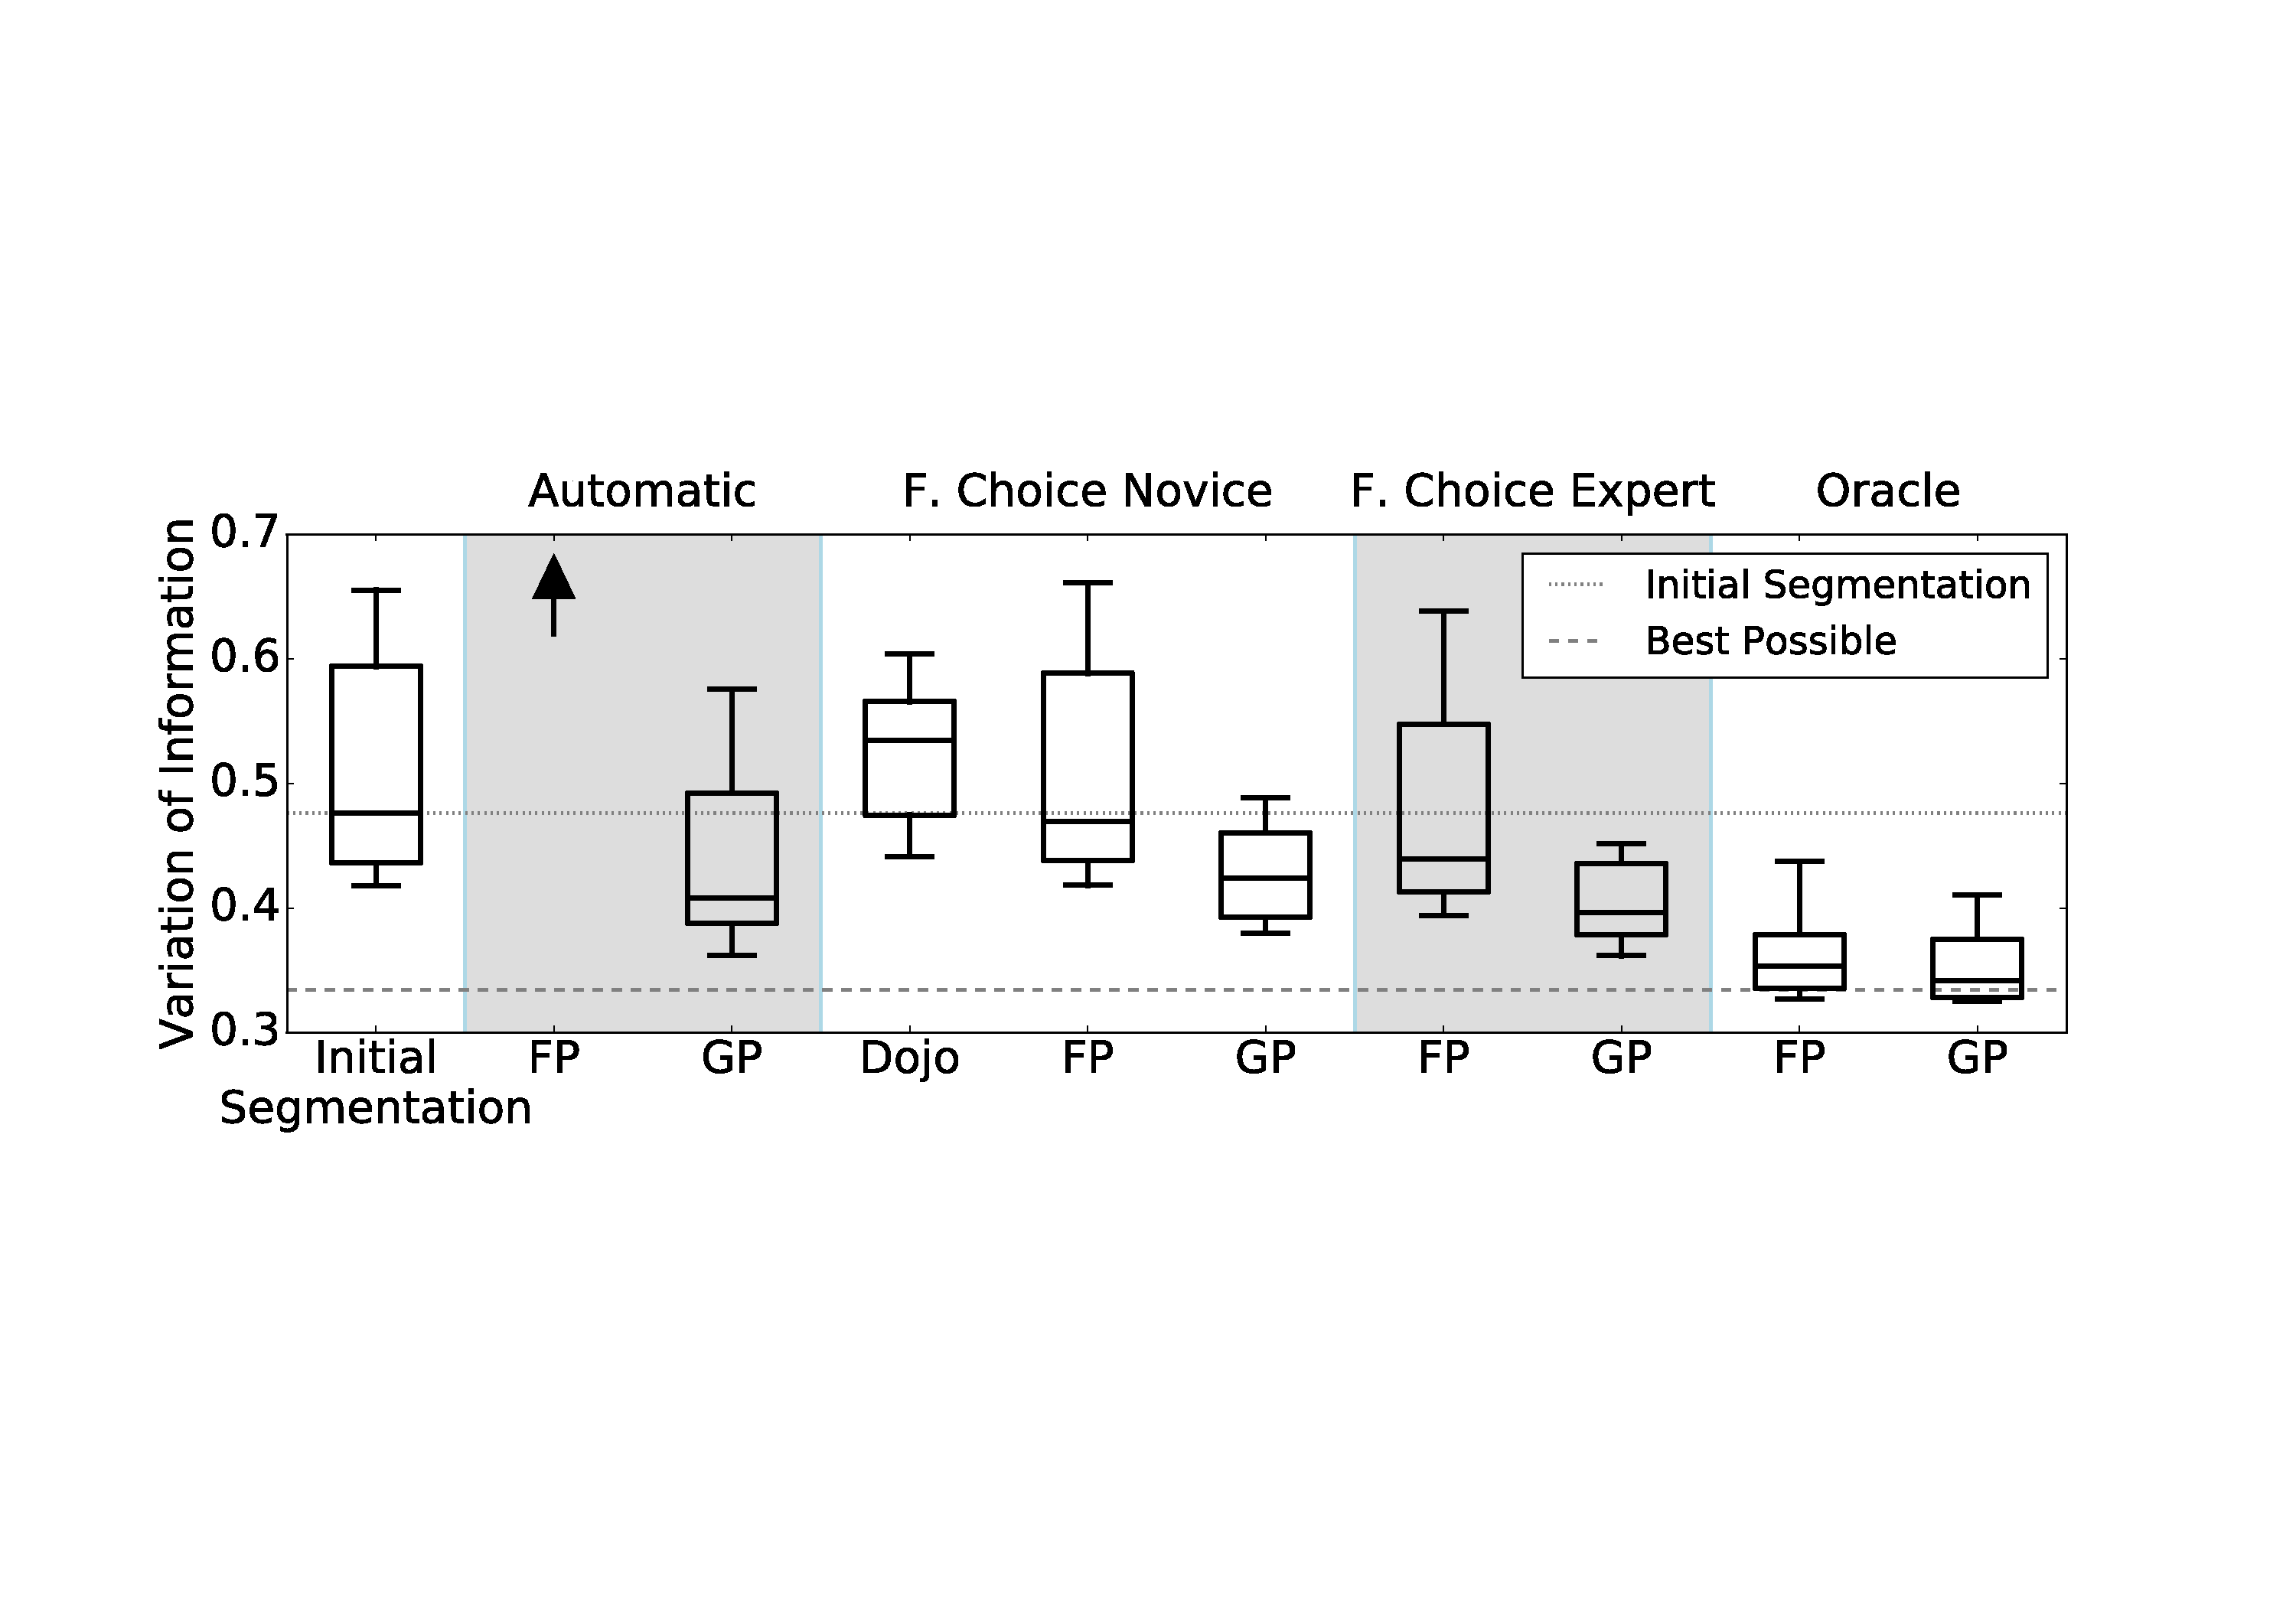
\includegraphics[width=\linewidth]{gfx/ac4boxplot.pdf}
\caption{VI distributions of guided proofreading (GP), focused proofreading (FP) and Dojo output across slices of the AC4 subvolume, with different error correction approaches. The variation resulting from performance of FP with automatic selection is $4.5\times$ higher than GP (as indicated by the arrow), with median VI of $1.9$ and $SD=0.496$.}
\label{fig:ac4boxplot}
\end{figure}

\subsection{Forced Choice User Experiment}
We performed a user study to evaluate the forced choice error correction method among novices and experts. To be comparable to Haehn~\etal's Dojo user study~\cite{haehn_dojo_2014}, participants were asked to proofread the AC4 subvolume for 30 minutes. We counted 10 merge errors and 322 split errors by computing the maximum overlap of the initial segmentation with respect to the ground truth labeling (provided in \cite{haehn_dojo_2014}). For evaluation, we measure the performance of proofreading quantitatively by comparing VI scores of segmentations. Median VI $=0.476$ ($SD=0.089$), with mean VI $=0.512$ ($SD=0.09$). Most novices and all experts were able to improve upon this score with both focused proofreading and guided proofreading (Fig.~\ref{fig:ac4trails}).

\paragraph{Novice performance.} Participants using focused proofreading were able to reduce the median VI of the automatic segmentation to $0.469$ ($SD=0.87$). On average, users viewed $423.4$ corrections and accepted $45.8$, with an average time of $4.9$ seconds per correction. Participants using guided proofreading were able to reduce the median VI to $0.424$ ($SD=0.037$). Here, users viewed on average $353.4$ corrections and accepted $106.9$, with an average correction time of $6.2$ seconds. While three users of focused proofreading made the initial segmentation worse, all participants using guided proofreading were able to improve it. In comparison to the results of Haehn~\etal, focused and guided proofreading outperform interactive proofreading with Dojo (median VI $0.535$, $SD=0.055$). The slope of VI score per correction (Fig.~\ref{fig:ac4trails}) shows that guided proofreading enables improvements with fewer corrections than the other tools. Interestingly, novice performance decreases after approximately $300$ corrections. There are two explanations for this: user fatigue, and increasing uncertainty during error suggestion from the classifier. %Regarding fatigue, we suggest that future experiments include short breaks after every ten minutes.

\paragraph{Expert performance.} Domain experts were able to improve the initial segmentation in all cases. With focused proofreading, the median VI of the automatic segmentation was $0.439$ ($SD=0.084$). With guided proofreading, the median VI was $0.396$ ($SD=0.032$, Fig.~\ref{fig:ac4boxplot}).

\paragraph{Subjective responses.} We used the NASA-TLX workload index to record subjective responses. Mental, physical, and temporal demands were reported slightly higher for participants using focused proofreading. However, these differences were not statistically significant. This is unsurprising as the user interface was the same for both groups.


\subsection{Automatic Error Correction}

\paragraph{Selection oracle.} As expected, the selection oracle yields the best performance on all datasets. Fig.~\ref{fig:ac4trails} shows VI reduction using the selection oracle on the AC4 subvolume (initial median VI $0.476$, $SD=0.089$). With focused proofreading, the selection oracle reaches a median VI of $0.353$ ($SD=0.037$) after $1600$ corrections. With guided proofreading, the oracle reaches a minimum median VI of $0.342$ ($SD=0.03$) after $800$ corrections. Both results are close to the best possible median VI of $0.334$ (calculated by computing maximum overlap with the ground truth). The slope of the trails in Fig.~\ref{fig:ac4trails} shows that guided proofreading requires fewer corrections to reach a reasonable reduction in VI. Fig.~\ref{fig:ac4boxplot} shows the VI distribution across methods. On the L.~Cylinder dataset (initial VI $0.379$, $SD=0.118$), focused proofreading reduces the median VI to $0.298$ ($SD=0.075$) after $26,170$ corrections ($2,419$ accepted). Guided proofreading reduces the median VI to $0.2996$ ($SD=0.073$) after $27,491$ corrections ($2,696$ accepted).

\paragraph{Automatic selection with threshold.} Focused proofreading was not designed to run automatically. This explains the poor performance on the AC4 subvolume (VI of $1.9$, $SD=0.496$) and on the L.~Cylinder dataset (VI of $2.75$, $SD=0.789$). For guided proofreading, we set $p_t=0.95$ for both datasets. This reduces median VI in the AC4 subvolume to $0.398$ ($SD=0.068$). This result is comparable to expert performance. Guided proofreading also reduces VI in the L.~Cylinder data to $0.352$ ($SD=0.087$).

\paragraph{Merge Error Detection.} Guided proofreading performs merge error detection prior to split error detection. The classifier found 10 merge errors in the AC4 subvolume, of which 4 reduced VI. Automatic selection with $p_t=0.95$ corrected 6 of these errors (Prec./Recall 0.87/0.80, F1-score 0.80). This was not captured in median VI, but resulted in a mean VI reduction from $0.512$ ($SD=0.09$) to $0.509$ ($SD=0.086$). The selection oracle reduced mean VI with only merge errors to $0.508$ ($SD=0.086$). In the forced choice user study, novices marked 1.9 merge errors for correction and reduced mean VI to $0.502$ (experts marked 2, VI $0.503$, $SD=0.086$). This shows how hard it is to identify merge errors. In 50 sections of the L.~Cylinder dataset, 151 merge errors were automatically found of which 17 reduced VI. Automatic selection with $p_t=0.95$ corrected 6 true VI-reducing errors and 30 VI-increasing ones (Prec./Recall 0.82/0.73, F1-score 0.77) to negligible VI effect. 

%\subsection{Limitations}
%Guided proofreading works on 2D image sections. This enables error correction without a computationally expensive alignment process. However, the output requires an additional (block-)merging step prior to 3D  analysis.
